\subsection{Results}
Figure \ref{fig-timePerTask} shows the time until the correct answer was given per task. Here we consider both the results from the controlled experiment as the online experiment, to remedy the small set of subjects available for the controlled experiment. We immediately see some interesting result for task 3. We do not know the underlying distribution so we perform a non-parametric Wilcoxon Mann-Whitney U test (\textit{$H_0$: times for the Console group and RxFiddle group are drawn from the same population}) to see if the differences are significant, and a Cliffs delta test for ordinal data to determine the effect size.

\begin{centering}
% \begin{table}[]
% \centering
% \caption{My caption}
%\label{my-label}
\begin{tabular}{llllll}
\hline
            & \textbf{$n_1$} & \textbf{$n_2$} & \textbf{W} & \textbf{p-value} & \textbf{Cliffs $\delta$} \\ \hline
\textbf{T1} & 26                      & 30                       & 343        & 0.448           & 0.121     \\
\textbf{T2} & 29                      & 27                       & 362        & 0.637           & 0.0754    \\
\textbf{T3} & 22                      & 24                       & 100        & 0.000186        & 0.621     \\
\textbf{T4} & 15                      & 12                       & 86         & 0.867           & 0.0444    \\ \hline
\end{tabular}
% \end{table}
\end{centering}

For tasks T3 we can reject $H_0$ with high significance ($p < 0.05$), the RxFiddle group is faster.
For the tasks T1, T2 and T4 we can not reject $H_0$ ($p > 0.05$), and for T2 the U test indicates no difference at all, meaning the RxFiddle group and Console group perform or could perform equally. While this could be observed as a negative result, RxFiddle is a new tool, and the users have only just been exposed to the tool and received only a short training. Of course it could also be the case  that RxFiddle might be more suitable to replace some tasks than others. From the results of the experiment we can not give a definitive explanation for the comparable results.

\begin{figure}[h]
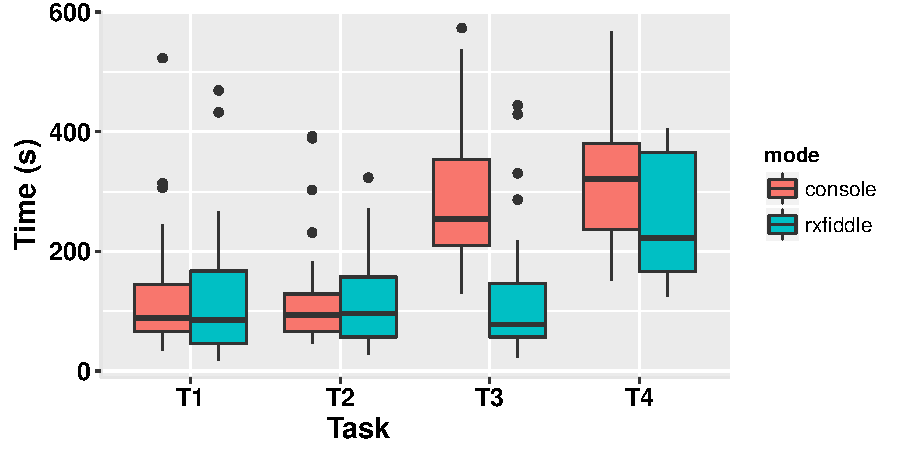
\includegraphics[width=\columnwidth]{images/timePerTask.pdf}
\caption{Time until correct answer per task}
\label{fig-timePerTask}
\end{figure}
